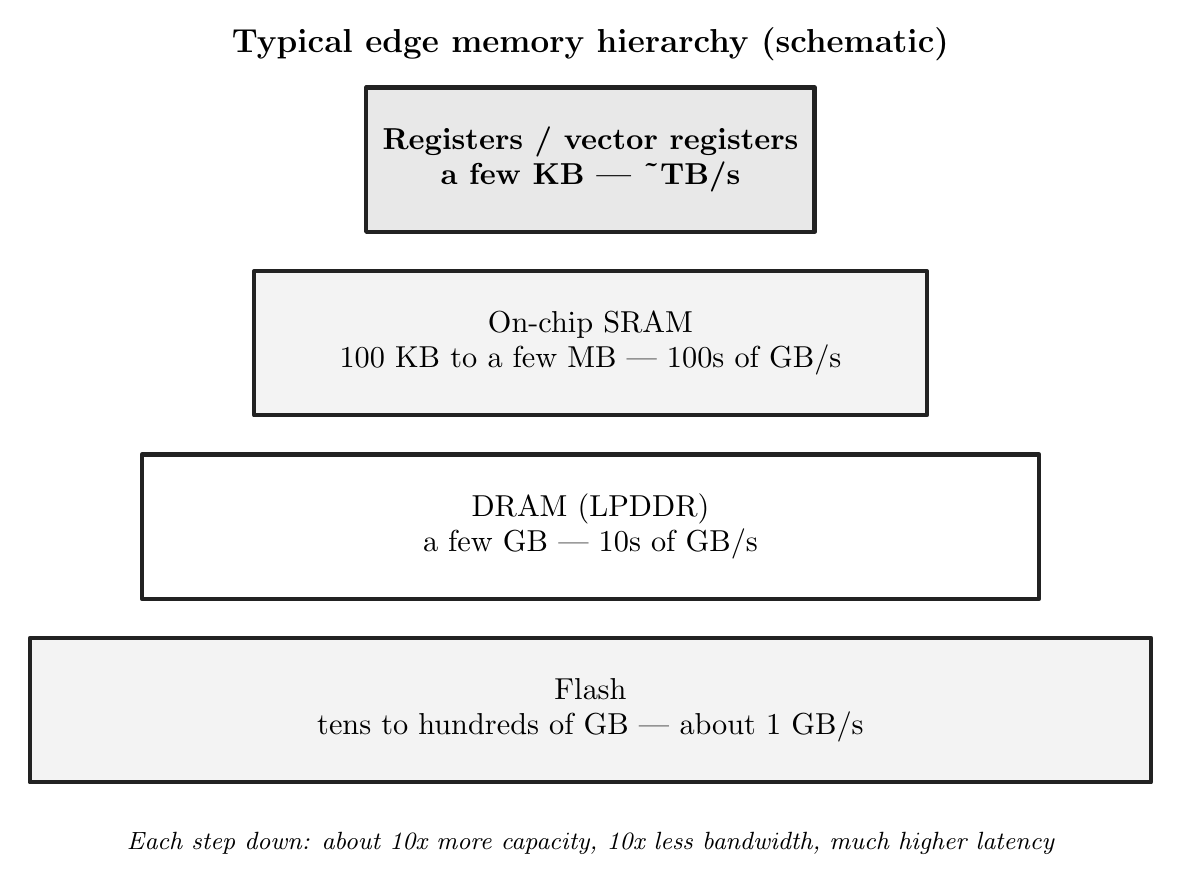
\begin{tikzpicture}[line cap=round,line join=round]
\draw[line width=1.58pt,draw={rgb,255:red,34;green,34;blue,34},fill={rgb,255:red,232;green,232;blue,232}] (1.979in,3.211in) rectangle (4.221in,3.932in);
\draw[line width=1.58pt,draw={rgb,255:red,34;green,34;blue,34},fill={rgb,255:red,243;green,243;blue,243}] (1.418in,2.294in) rectangle (4.782in,3.014in);
\draw[line width=1.58pt,draw={rgb,255:red,34;green,34;blue,34},fill={rgb,255:red,255;green,255;blue,255}] (0.857in,1.376in) rectangle (5.343in,2.097in);
\draw[line width=1.58pt,draw={rgb,255:red,34;green,34;blue,34},fill={rgb,255:red,243;green,243;blue,243}] (0.297in,0.459in) rectangle (5.903in,1.180in);
\node[align=center,text={rgb,255:red,0;green,0;blue,0},font=\fontsize{10.6pt}{12.6pt}\selectfont\bfseries,inner sep=0pt] at (3.100in,3.571in) {Registers / vector registers \\ a few KB  |  \textasciitilde{}TB/s};
\node[align=center,text={rgb,255:red,0;green,0;blue,0},font=\fontsize{10.6pt}{12.6pt}\selectfont,inner sep=0pt] at (3.100in,2.654in) {On-chip SRAM \\ 100 KB to a few MB  |  100s of GB/s};
\node[align=center,text={rgb,255:red,0;green,0;blue,0},font=\fontsize{10.6pt}{12.6pt}\selectfont,inner sep=0pt] at (3.100in,1.737in) {DRAM (LPDDR) \\ a few GB  |  10s of GB/s};
\node[align=center,text={rgb,255:red,0;green,0;blue,0},font=\fontsize{10.6pt}{12.6pt}\selectfont,inner sep=0pt] at (3.100in,0.819in) {Flash \\ tens to hundreds of GB  |  about 1 GB/s};
\node[anchor=south,align=center,text={rgb,255:red,0;green,0;blue,0},font=\fontsize{11.5pt}{13.6pt}\selectfont\bfseries,inner sep=0pt] at (3.100in,4.063in) {Typical edge memory hierarchy (schematic)};
\node[anchor=south,align=center,text={rgb,255:red,0;green,0;blue,0},font=\fontsize{9.4pt}{11.0pt}\selectfont\itshape,inner sep=0pt] at (3.100in,0.098in) {Each step down: about 10x more capacity, 10x less bandwidth, much higher latency};
\end{tikzpicture}
